% Written by Louise Fussien

% This file CAN NOT be compiled on its own
% It is included by ../Book_of_Specifications.tex

\subsection{Analyse et progrès}

\subsubsection*{Status actuel}


Nous sommes heureux de confirmer que le développement de Lands of Azerith est terminé dans son intégralité. Tous les éléments du jeu ont été entièrement implémentés et rigoureusement testés pour garantir une expérience de jeu optimale. Voici un récapitulatif des principales réalisations :
\\

\begin{itemize}

    \item Scénario complet : Le jeu est structuré en trois actes, chacun divisé en 5 à 7 parties, avec une histoire riche et immersive. Chaque acte est complètement jouable et offre une progression narrative captivante.
    \\

    \item Zones de jeu : Les 21 zones distinctes, chacune représentant un biome unique, ont été entièrement développées. Chaque zone a été soigneusement conçue pour offrir des environnements diversifiés et détaillés.
    \\

    \item Classes de personnage : Les neuf classes de personnage sont finalisées et équilibrées, offrant aux joueurs une variété de styles de jeu et de compétences uniques.
    \\

    \item Système de combat : Les mécaniques de combat, y compris les compétences, pouvoirs élémentaires, armes et consommables, ont été entièrement implémentées et optimisées pour une jouabilité fluide et   engageante.
    \\

    \item Quêtes : Toutes les quêtes principales et secondaires sont en place, offrant une variété de défis et de récompenses. Les quêtes secondaires influencent également les fins possibles du jeu.
    \\

    \item Boss et donjons : Tous les boss, y compris ceux des donjons et des zones ouvertes, sont intégrés et offrent des défis adaptés au niveau de progression du joueur.
    \\

    \item Multijoueur : Le mode multijoueur est opérationnel.
    \\

    \item Design et son : Tous les éléments visuels et sonores ont été finalisés, avec une attention particulière à l'immersion et à l'esthétique du jeu.
    \\

\end{itemize}

\subsubsection*{Délais rencontrés et raisons}

Nous avons rencontré des retards principalement dus aux changements des membres du groupe et à des défis techniques imprévus. 
Par exemple, l'intégration des systèmes de quête secondaire a nécessité plus de temps que prévu en raison de la complexité de l'interaction entre les différentes quêtes et leur impact potentiel sur l'histoire principale.
\\

\subsection{Organisation du groupe}

\subsubsection{Tâches attribuées}

Pour assurer une collaboration efficace au sein de notre groupe de projet, nous avons opté pour l'utilisation de plusieurs outils de communication. 
Principalement, nous avons utilisé Discord, une plateforme de communication instantanée, pour faciliter les échanges en temps réel entre les membres du groupe. 
Discord nous a permis de maintenir une communication fluide et réactive, essentielle pour coordonner nos efforts et résoudre rapidement les problèmes rencontrés pendant le développement du projet. 
Les fonctionnalités de chat vocal et textuel de Discord ont été particulièrement utiles pour organiser des réunions spontanées et des discussions en groupe, améliorant ainsi notre efficacité collaborative.
\\

En complément de Discord, nous avons également profité des sessions de travail en groupe en présentiel sur le campus. 
ces rencontres physiques nous ont offert l'opportunité de discuter en profondeur des aspects techniques et conceptuels du projet, de partager des idées de manière plus interactive et de travailler sur des tâches spécifiques ensemble. 
Cette combinaison d'interactions en ligne via Discord et en personne sur le campus nous a permis de tirer parti des avantages uniques de chaque mode de communication, renforçant ainsi notre cohésion d'équipe et notre efficacité dans l'accomplissement des objectifs du projet.
\\

\subsubsection{GitHub}

Github a joué un rôle central dans la gestion et le partage de notre code source tout au long du projet. 
Nous avons utilisé GitHub comme plateforme principale pour héberger notre repository de projet, ce qui nous a permis de collaborer efficacement sur le code. 
Chaque membre du groupe a pu créer des branches de développement distinctes pour travailler sur des fonctionnalités spécifiques sans perturber la branche principale, tout en utilisant des pull requests pour fusionner les contributions et effectuer des révisions par les pairs.
\\

L'intégration de GitHub avec notre flux de travail nous a offert plusieurs avantages. 
Premièrement, cela a facilité la gestion des versions du code et le suivi des modifications apportées à mesure que le projet évoluait. 
Deuxièmement, GitHub a facilité la détection et la résolution des conflits de fusion, assurant ainsi l'intégrité du code source partagé entre les membres du groupe. 
\\

\subsubsection{Cahier des charges techniques}
% This file CAN NOT be compiled on its own
% It is included by ../Book_of_Specifications.tex

% TODO Update the technical book

Les deux prochaines pages sont dédiées au cahier des charges technique.
Ce document détaille les contraintes et les caractéristiques techniques nécessaires pour répondre aux besoins du projet.
Il synthétise toutes les réponses aux questions techniques que l'on peut se poser sur le projet.
\\

Le cahier des charges technique est divisé en deux parties.
La première partie détaille les spécificités du jeu et les choix techniques qui ont été réalisés. 
La deuxième partie donne des informations sur la repartition des tâches et leur avancement.
\\

Des changements ont été apportés au cahier des charges technique depuis sa dernière version.
Le nom du jeu a été modifié, le départ de Mohamed Aziz et Alexandre a été pris en compte, et des changements ont été apportés au diagramme de Gantt pour refléter l'avancé du projet.
\\

Le dernier cahier des charges technique, intégré dans ce rapport final, reflète ces ajustements. Il décrit non seulement 
les spécifications finales du jeu telles qu'elles ont évolué tout au long du processus, mais aussi les décisions stratégiques prises pour surmonter les défis rencontrés.



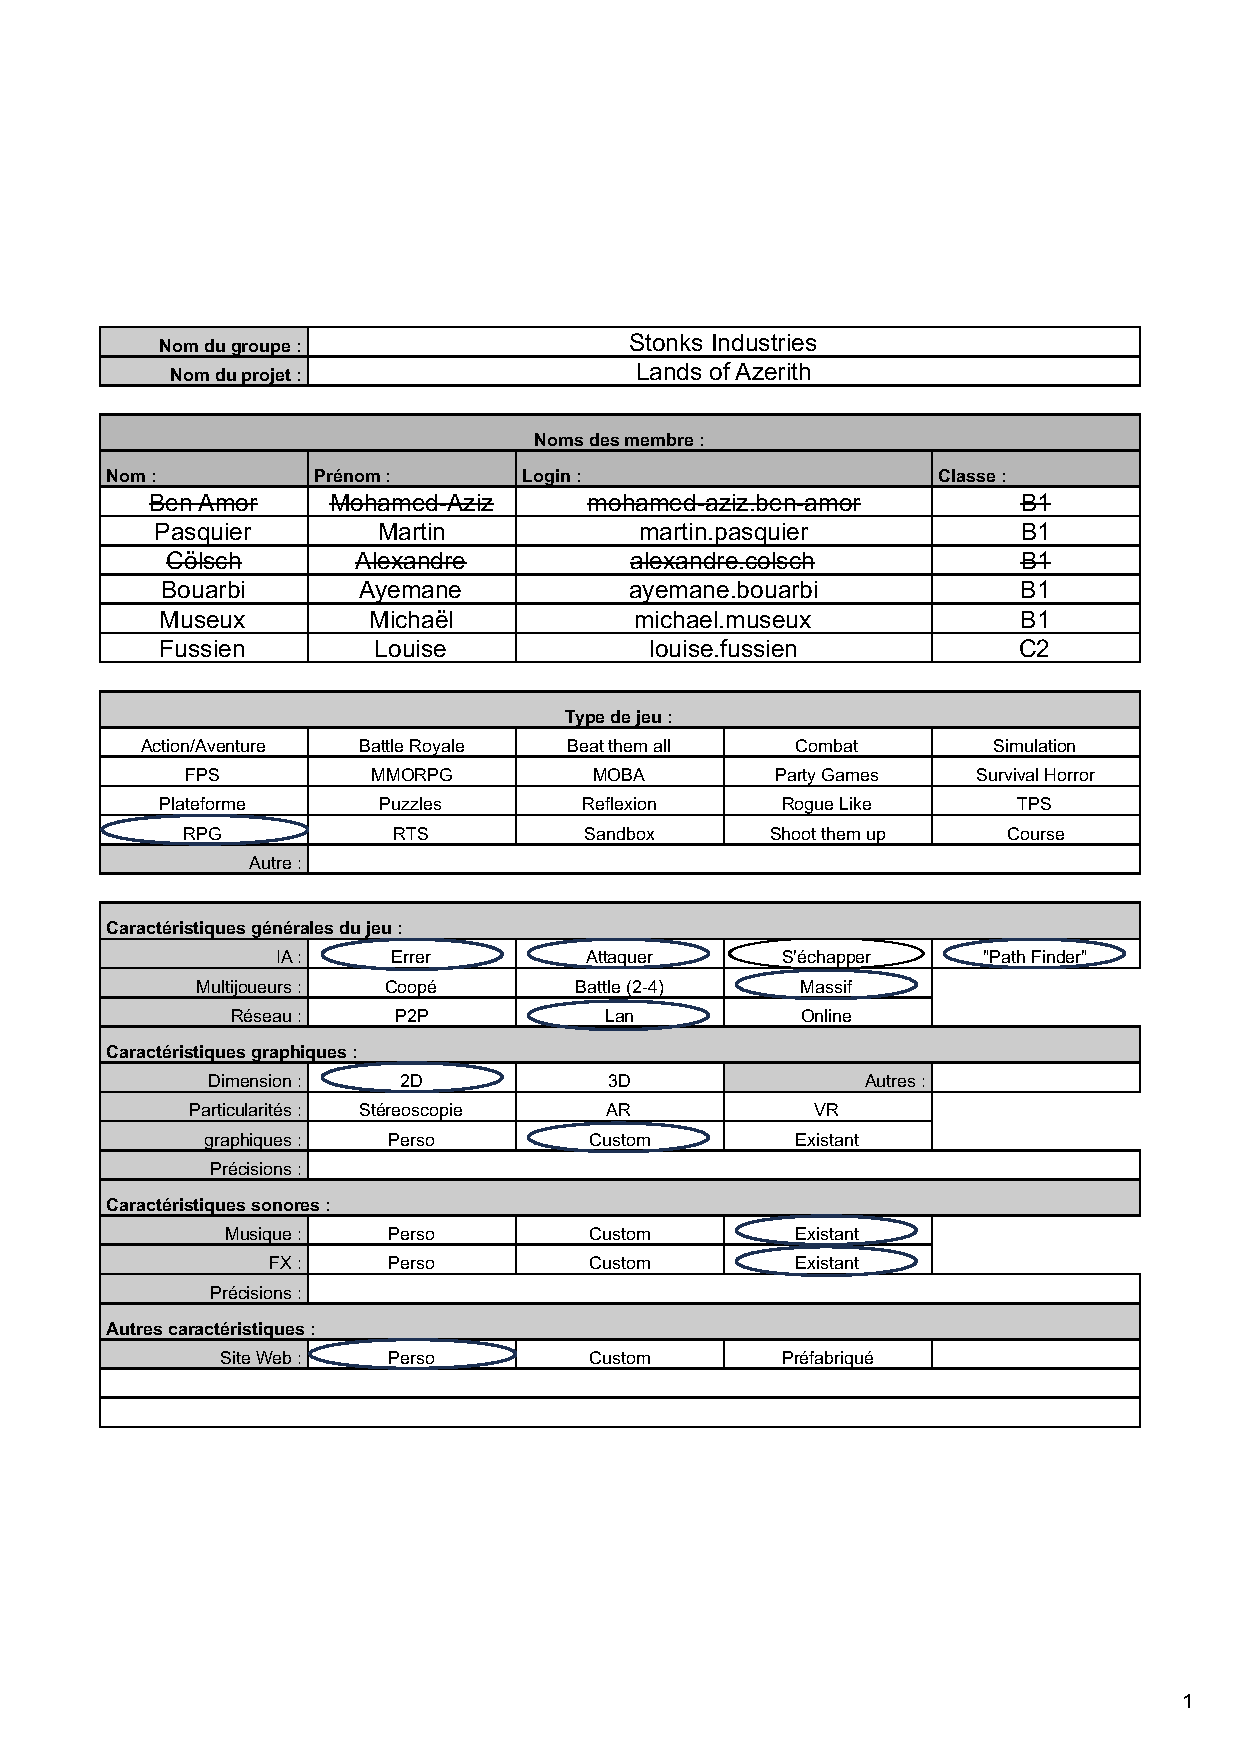
\includepdf[pages=1]{technical_book/page-1.pdf}

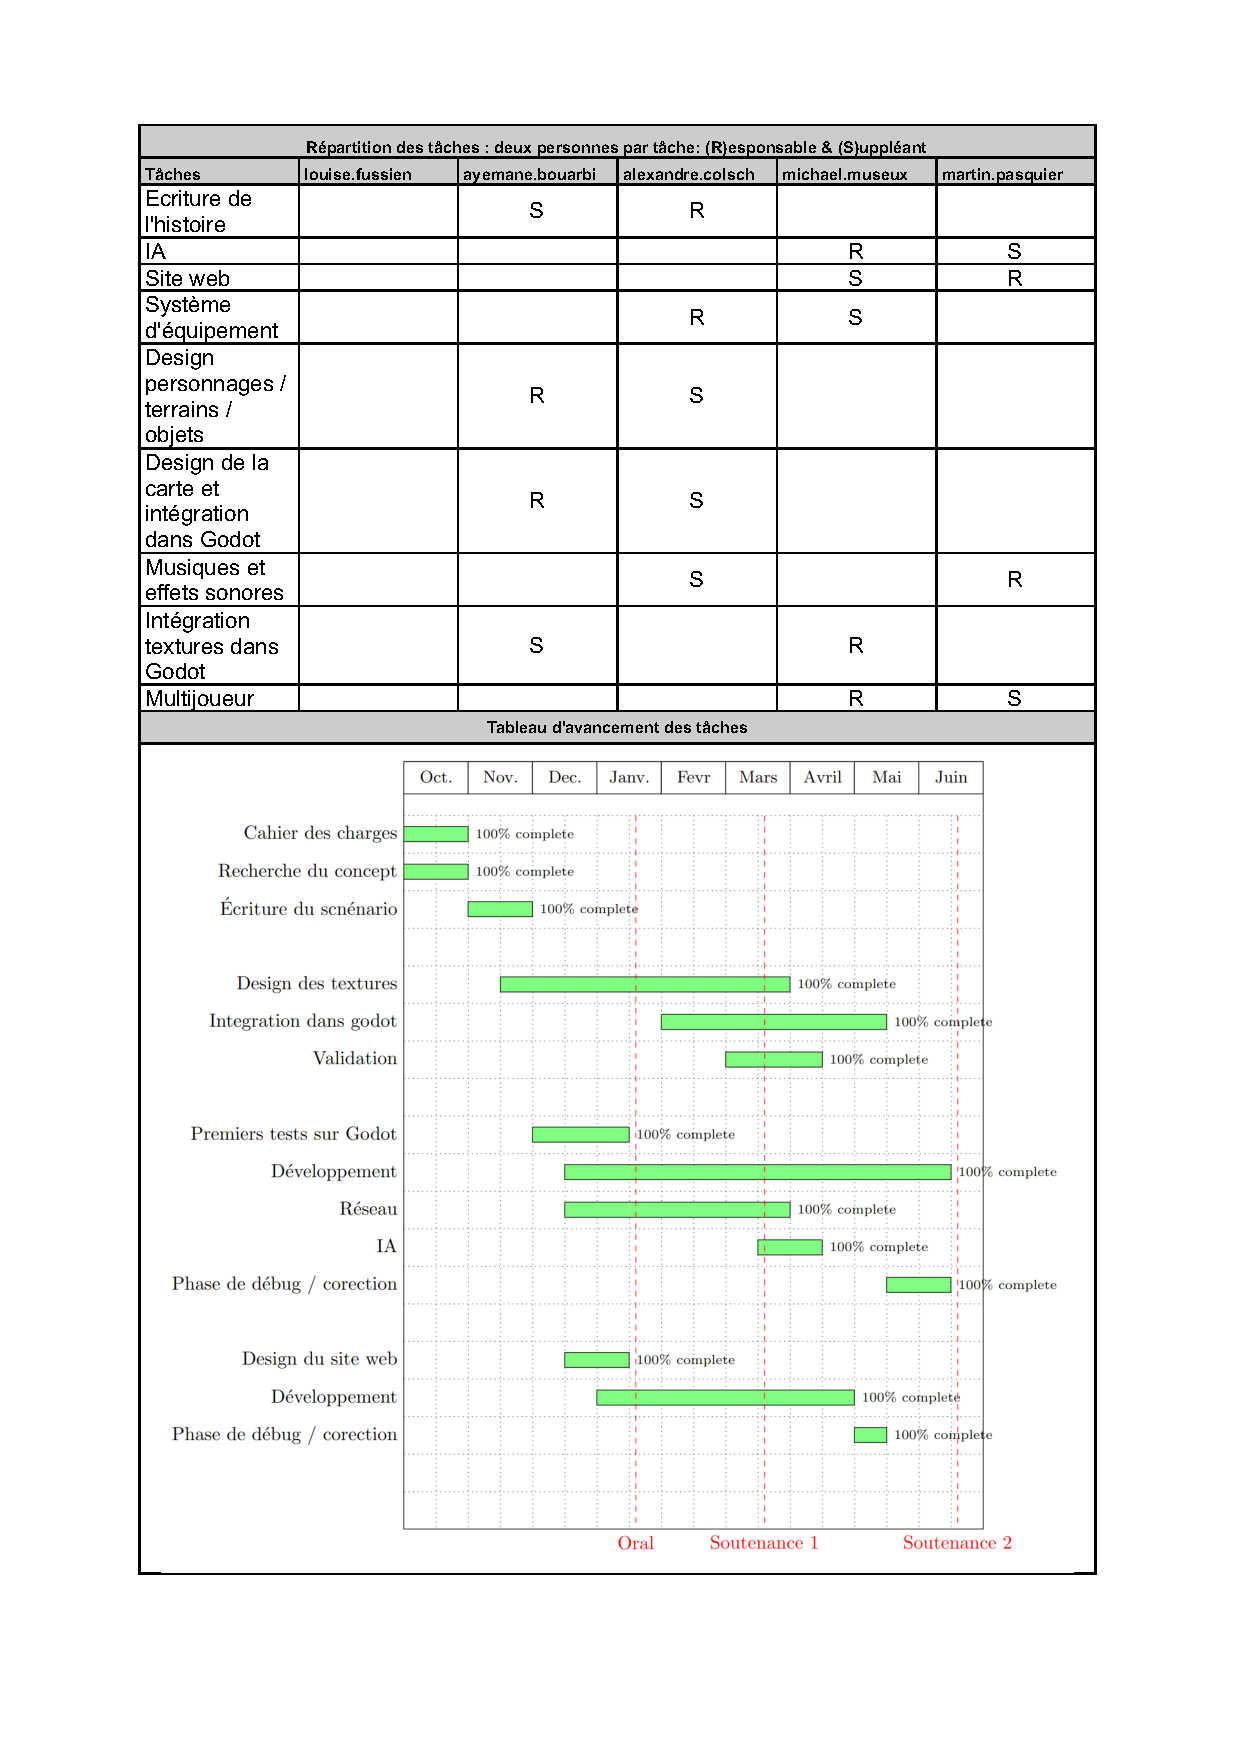
\includepdf[pages=1]{technical_book/page-2.pdf}

